% !TEX encoding = IsoLatin                     
%cette premiÃère ligne permet au compilateur (souvent, dÃépend du compilateur) \LaTeX de reconnaitre l'encodage de votre fichier. 
%\documentclass[12pt,titlepage,twoside]{book}       %pour un livre
%\documentclass{report}
\documentclass[a3, 10pt,twoside]{article}          %pour un article
%\documentclass[twocolumn,amsfonts,showpacs,superscriptaddress,nofootinbib,aps,nolongbibliography]{revtex4-2}
%\documentclass[onecolumn,amsfonts,showpacs,superscriptaddress]{revtex4-1}

\usepackage{array,multirow,graphicx}
\usepackage[T1]{fontenc}  % For correct {}s in \texttt
\usepackage{accents}
\usepackage[francais]{babel}
\usepackage{amssymb, amssymb, amsthm}
\usepackage[utf8]{inputenc}             
\usepackage{amstext, amsfonts, a4}
\usepackage{pgf,pgfarrows,pgfautomata,pgfheaps,pgfnodes,pgfshade}
\usepackage[left=0.05cm,right=0.05cm,top=0.05cm,bottom=0.05cm,nohead]{geometry}
\usepackage{natbib}
%\usepackage{amsmath,amssymb}
\usepackage[pdfborder={0 0 0}]{hyperref}
\usepackage{xxcolor}
\usepackage{amscd}
\usepackage{dsfont}
\usepackage{float} 
\usepackage[Glenn]{fncychap} % Rejne Glenn\chapter
%\usetikzlibrary{circuits.ee.IEC}
\usepackage{lipsum} % pour générer du texte aléatoire

%\usepackage[tikz]{bclogo}
\usepackage{mathrsfs}%lagrangien
\usepackage{stmaryrd} %\llbracket
\usepackage{bbold}%Matrice 11
\usepackage{shapepar}
\usepackage{cancel}
\usepackage{bm}
\usepackage{pdfpages}
\usepackage[utf8]{inputenc}
\usepackage{marvosym}
\usepackage{enumitem}
\usepackage{import} % Charger le package import
\usepackage{listings} % Pour afficher du code MATLAB
\usepackage{pgfplots}
\usetikzlibrary {datavisualization}
\usetikzlibrary {arrows.meta,bending,positioning}
\usetikzlibrary {datavisualization.formats.functions}

\usepackage{tikz}
\usepackage[europeanresistor]{circuitikz}
\usepgflibrary {shadings}
%\usetikzlibrary{calc}
\usetikzlibrary{hobby, decorations.markings, arrows.meta}
\usetikzlibrary{decorations.markings} 
\usetikzlibrary{calc,intersections,through,backgrounds}
\usetikzlibrary {arrows.meta}


%%%%%%%%%%%%%%%%%%%%%%%%%%%%%%%%% Pour le tag
%\usepackage[utf8]{inputenc}
%\usepackage{fourier}
\usepackage{mathtools}
%\usepackage{cleveref}
\usepackage{xcolor}
%%%%%%%%%%%%%%%%%%%%%%%%%%%%%%%%%%


%%%%%%%%%%%%%%%%%%%%%%%%%%%%%%%%%%
\newcommand{\operatorvec}[1]{\hat{{\bm{#1}}}} % pour les operateur
\newcommand{\operator}[1]{\hat{\bm{#1}}} % pour les operaeur vecteur 
\newcommand{\operatortilde}[1]{\tilde{\bm{#1}}} % pour les opetateur avec un tilde
\newcommand{\operatortildevec}[1]{\tilde{\bm{#1}}}% pour les opetateur avec un tilde et vecteur 
%%%%%%%%%%%%%%%%%%%%%%%%%%%%%%%%%%

%\usepackage{tzplot}

%\usepakage{pstriks}
\usepackage[utf8]{inputenc}

%PREAMBULE pour schÃéma
\usepackage{pgfplots}
\usepackage{tikz}
%\usepackage[european resistor, european voltage, european current]{circuitikz}
%\usetikzlibrary{arrows,shapes,positioning}
%\usetikzlibrary{decorations.markings,decorations.pathmorphing,decorations.pathreplacing}
%\usetikzlibrary{calc,patterns,shapes.geometric}
\usetikzlibrary{patterns} % Pour les motifs comme les lignes diagonales
\usepackage{float} % Pour le placement 'H'
%FIN PREAMBULE

% PREAMBULE pour vercteur derivÃé
\usepackage[b]{esvect}    % For \vv

%\usepackage{caption}
%\usepackage{subcaption}

%\usepackage{graphicx}

\usepackage{fullpage}
\usepackage{eso-pic}
\usepackage{enumitem}

%\usepackage{pgfplots}
%\pgfplotsset{compat=1.17}



% --- Macro \xvec
\makeatletter
\newlength\xvec@height%
\newlength\xvec@depth%
\newlength\xvec@width%
\newcommand{\xvec}[2][]{%
  \ifmmode%
    \settoheight{\xvec@height}{$#2$}%
    \settodepth{\xvec@depth}{$#2$}%
    \settowidth{\xvec@width}{$#2$}%
  \else%
    \settoheight{\xvec@height}{#2}%
    \settodepth{\xvec@depth}{#2}%
    \settowidth{\xvec@width}{#2}%
  \fi%
  \def\xvec@arg{#1}%
  \def\xvec@dd{:}%
  \def\xvec@d{.}%
  \raisebox{.2ex}{\raisebox{\xvec@height}{\rlap{%
    \kern.05em%  (Because left edge of drawing is at .05em)
    \begin{tikzpicture}[scale=1]
    \pgfsetroundcap
    \draw (.05em,0)--(\xvec@width-.05em,0);
    \draw (\xvec@width-.05em,0)--(\xvec@width-.15em, .075em);
    \draw (\xvec@width-.05em,0)--(\xvec@width-.15em,-.075em);
    \ifx\xvec@arg\xvec@d%
      \fill(\xvec@width*.45,.5ex) circle (.5pt);%
    \else\ifx\xvec@arg\xvec@dd%
      \fill(\xvec@width*.30,.5ex) circle (.5pt);%
      \fill(\xvec@width*.65,.5ex) circle (.5pt);%
    \fi\fi%
    \end{tikzpicture}%
  }}}%
  #2%
}
\makeatother

% --- Override \vec with an invocation of \xvec.
\let\stdvec\vec
\renewcommand{\vec}[1]{\xvec[]{#1}}
% --- Define \dvec and \ddvec for dotted and double-dotted vectors.
\newcommand{\dvec}[1]{\xvec[.]{#1}}
\newcommand{\ddvec}[1]{\xvec[:]{#1}}
% FIN PREAMBULE


\def\pgf{\textsc{pgf}}
\def\pstricks{\textsc{pstricks}}
\def\Class#1{\hbox{\small#1}}
\def\bs{$\backslash$}

\def\Environment#1{\par\bigskip\noindent\textbf{Environment \texttt{#1}}\par}
\def\Command#1{\par\bigskip\noindent\textbf{Command \texttt{#1}}\par}
\long\def\Parameters#1{\medskip\noindent Parameters:
  \begin{enumerate}\itemsep=0pt\parskip=0pt
    #1
  \end{enumerate}}
\long\def\Description#1{\unskip\medskip\noindent Description: #1}
\def\Example{\par\medskip\noindent Example: }


\renewcommand*\descriptionlabel[1]{\hspace\labelsep\normalfont #1}


\def\declare#1{{\color{red!75!black}#1}}

\def\command#1{\list{}{\leftmargin=2em\itemindent-\leftmargin\def\makelabel##1{\hss##1}}%
\item\extractcommand#1@\par\topsep=0pt}
\def\endcommand{\endlist}
\def\extractcommand#1#2@{\strut\declare{\texttt{\string#1}}#2}


\def\environment#1{\list{}{\leftmargin=2em\itemindent-\leftmargin\def\makelabel##1{\hss##1}}%
\extractenvironement#1@\par\topsep=0pt}
\def\endenvironment{\endlist}
\def\extractenvironement#1#2@{%
\item{{\ttfamily\char`\\begin\char`\{\declare{#1}\char`\}}#2}%
  {\itemsep=0pt\parskip=0pt\item{\meta{environment contents}}%
  \item{\ttfamily\char`\\end\char`\{\declare{#1}\char`\}}}}


\def\smallpackage{\vbox\bgroup\package}
\def\endsmallpackage{\egroup\endpackage}
\def\package#1{\list{}{\leftmargin=2em\itemindent-\leftmargin\def\makelabel##1{\hss##1}}%
\extracttheme#1@\par\topsep=0pt}
\def\endpackage{\endlist}
\def\extracttheme#1#2@{%
\item{{{\ttfamily\char`\\usepackage}#2{\ttfamily\char`\{\declare{#1}\char`\}}}}}



\def\Environment#1{\par\bigskip\noindent\textbf{Environment \texttt{#1}}\par}
\def\Command#1{\par\bigskip\noindent\textbf{Command \texttt{#1}}\par}
\long\def\Parameters#1{\medskip\noindent Parameters:
  \begin{enumerate}\itemsep=0pt\parskip=0pt
    #1
  \end{enumerate}}
\long\def\Description#1{\unskip\medskip\noindent Description: #1}
\def\Example{\par\medskip\noindent Example: }

\newcommand{\w}[1]{\bf{#1}}\newcommand{\ww}[1]{\bf{#1}}
%\newcommand{\w}[1]{\vec{#1}}\newcommand{\ww}[1]{\overrightarrow{#1}}



\newcommand{\vertiii}[1]{{\left\vert\kern-0.25ex\left\vert\kern-0.25ex\left\vert#1\right\vert\kern-0.25ex\right\vert\kern-0.25ex\right\vert}}

%%%%%%%%%%%%%%%%%%%%%%%%%%%%%%%%%%%%%%%%%%%%%%%%%%%%%%%%%%%
    %%%%%%%% Accent Math
%%%%%%%%%%%%%%%%%%%%%%%%%%%%%%%%%%%%%%%%%%%%%%%%%%%%%%%%%%%
\makeatletter
\newcommand*{\math@auxii}[2][3]{{}\mkern#1mu\overline{\mkern-#1mu#2}}
\newcommand*{\math@auxi}[3][3]{\overset{\mkern#1mu\text{\scalebox{0.7}{#3}}\mkern-#1mu}{\smash{\math@auxii[#1]{#2}}\vphantom{#2}}}
\newcommand*{\mathco}[2][3]{\math@auxi[#1]{#2}{$\circ$}}
\newcommand*{\mathabc}[2][3]{\math@auxi[#1]{#2}{abc}}
\makeatother

%%%%%%%%%%%%%%%%%%%%%%%%%%%%%%%%%%%%%%%%%%%%%%%%%%%%%%%%%
%%%%algorithmes / pseudo code%%%
%%%%%%%%%%%%%%%%%%%%%%%%%%%%%%%%%%%%%%%%%%%%%%%%%%%%%%%%%%
\usepackage[french,ruled]{algorithm2e}

%%%%%
\usepackage{color,transparent}
%%%%%
%\usepackage{graphics,graphicx,subfigure,caption}
%\usepackage{graphics,graphicx,caption}
\usepackage{caption}
\usepackage{subcaption}
\usepackage{comment}
\usepackage{float} 
\setcounter{MaxMatrixCols}{30}%

%%%%%%%%%%%%%%%%%%%%%%%%%%%%%%%%%%%%%%%%
%%%%        Dimensions du texte (à adapter selon votre goût/le goût de l'Ãéditeur)
%%%%%%%%%%%%%%%%%%%%%%%%%%%%%%%%%%%%%%%%

\setlength\textwidth{19cm}          % largeur du texte
\setlength\topmargin{-1cm}          % marge en haut
\setlength\evensidemargin{-1cm}     % marge de gauche
\setlength\textheight{24cm}         % hauteur du texte
\setlength\oddsidemargin{\evensidemargin}

%%%%%%%%%%%%%%%%%%%%%%%%%%%%%%%%%%%%%%%%
%         D\'ecoupage des mots           %
%%%%%%%%%%%%%%%%%%%%%%%%%%%%%%%%%%%%%%%%
\hyphenation{}

%%%%%%%%%%%%%%%%%%%%%%%%%%%%%%%%%%%%%%%%
%%%%  Th\'eor\`emes, d\'efinitions, etc.
%%%%%%%%%%%%%%%%%%%%%%%%%%%%%%%%%%%%%%%%


% Il y a diffÃérents types d'ÃénoncÃés qui mÃéritent un environnement spÃécifique, voici une liste assez exhaustive. 
\theoremstyle{plain}
	\newtheorem{Theo}{Th\'eor\`eme}[section] %compteur commençant par le numÃéro de la section (on pourrait aussi faire commencer par le numÃéro de la sous-section - remplacer "section" par "subsection")
	\newtheorem{Prop}[Theo]{Proposition}        %mÃême compteur que pour les thÃéorÃèmes      
	\newtheorem{Prob}[Theo]{Probl\`eme}	    %idem
	\newtheorem{Lemm}[Theo]{Lemme}            %etc...
	\newtheorem{Coro}[Theo]{Corollaire}
	\newtheorem{Propr}[Theo]{Propri\'et\'e}
	\newtheorem{Conj}[Theo]{ Conjecture}
	\newtheorem{Aff}[Theo]{Affirmation}

    \newtheorem{TheoPrinc}{Th\'eor\`eme}     %compteur spÃécifique pour les thÃéorÃèmes les plus importants du papier
        
\theoremstyle{definition}
	\newtheorem{Defi}[Theo]{D\'efinition}
    \newtheorem{Exem}[Theo]{Exemple}
	\newtheorem{Nota}[Theo]{\Large Notation}

\theoremstyle{remark}
	\newtheorem{Rema}[Theo]{Remarque}
	\newtheorem{NB}[Theo]{N.B.}
	\newtheorem{Comm}[Theo]{Commentaire}
	\newtheorem{question}[Theo]{$\ast$ Question}
	\newtheorem{exer}[Theo]{Exercice}
	\newtheorem{Consequence}[Theo]{Conséquence}
	\newtheorem{Rap}[Theo]{Rappel}
	\newtheorem*{Merci}{Remerciements}
	
\usepackage{mdframed}

\mdfdefinestyle{propstyle}{%
linecolor=black,linewidth=2pt,%
hidealllines=true,
frametitlerule=true,%
frametitlebackgroundcolor=gray!20,
backgroundcolor=gray!10!white,
roundcorner=5pt,
innertopmargin=\topskip,
}

%\mdtheorem[style=propstyle]{prop}{Property}[chapter]
\mdtheorem[style=propstyle]{lemma}[prop]{Lemma}
\mdtheorem[style=propstyle]{TheoPrinc}{Th\'eor\`eme}[chapter]

% Définition d'un style personnalisé pour les Affirmations
\mdfdefinestyle{affirmestyle}{%
    linecolor=gray, % Couleur de la bordure
    linewidth=1pt, % Épaisseur de la bordure
    backgroundcolor=gray!10, % Couleur de fond (gris clair)
    roundcorner=5pt, % Coins arrondis
    innertopmargin=\topskip, % Marge intérieure
    skipabove=10pt, % Espace au-dessus du cadre
    skipbelow=10pt % Espace en-dessous du cadre
}

% Définition de l'environnement Affirmation
\theoremstyle{definition} % Style de théorème pour les affirmations
\newmdtheoremenv[style=affirmestyle]{aff}{Affirmation} % Environnement Affirmation avec le style personnalisé


	

%%%%%%%%%%%%%%%%%%%%%%%%%%%%%%%%%%%%%%%%
%%%%  Accolades, guillemets, etc.
%%%%%%%%%%%%%%%%%%%%%%%%%%%%%%%%%%%%%%%%

\def\ogg~{{\rm \og}}   % guillemets ouvrants
\def\fgg{{\rm \fg}}  % guillemets fermants



\def\nl{\newline}
\def\nn{\noindent}

\def\q{\nn}
\def\qq{\nn\quad}
\def\qqq{\nn\quad\quad}
\def\qqqq{\nn\quad\quad\quad}
\def\ce{\centerline}

%%%%%%%%%%%%%%%%%%%%%%%%%%%%%%%%%%%%%%%%
%%%%  Lettres et symboles math\'ematiques
%%%%%%%%%%%%%%%%%%%%%%%%%%%%%%%%%%%%%%%%

\def\emptyset{\varnothing}

%%%% Raccourcis pour les caractÃères gras mathÃématiques (ensembles R, N, Z, C etc)

\def\NN{{\mathbb N}}    %naturels
\def\ZZ{{\mathbb Z}}     %entiers relatifs
\def\RR{{\mathbb R}}    %rÃéels
\def\QQ{{\mathbb Q}}    %rÃéels
\def\CC{{\mathbb C}}    %complexes
\def\HH{{\mathbb H}}    %quaternions / espace hyperbolique
\def\AA{{\mathbb P}}     %espace projectif
\def\KK{{\mathbb K}}     %corps quelconques

\def\EE{{\mathbb E}}     %Experance
\def\VV{{\mathbb V}}     %Variance

%%%%%%raccourcis lettres calligraphiÃées
\def\cA{{\mathcal A}}  \def\cG{{\mathcal G}} \def\cM{{\mathcal M}} \def\cS{{\mathcal S}} \def\cB{{\mathcal B}}  \def\cH{{\mathcal H}} \def\cN{{\mathcal N}} \def\cT{{\mathcal T}} \def\cC{{\mathcal C}}  \def\cI{{\mathcal I}} \def\cO{{\mathcal O}} \def\cU{{\mathcal U}} \def\cD{{\mathcal D}}  \def\cJ{{\mathcal J}} \def\cP{{\mathcal P}} \def\cV{{\mathcal V}} \def\cE{{\mathcal E}}  \def\cK{{\mathcal K}} \def\cQ{{\mathcal Q}} \def\cW{{\mathcal W}} \def\cF{{\mathcal F}}  \def\cL{{\mathcal L}} \def\cR{{\mathcal R}} \def\cX{{\mathcal X}} \def\cY{{\mathcal Y}}  \def\cZ{{\mathcal Z}}

%%%%%%raccourcis lettres gothiques

\def\mfA{{\mathfrak A}} \def\mfA{{\mathfrak P}} \def\mfS{{\mathfrak S}}\def\mfZ{{\mathfrak Z}} \def\mfM{{\mathfrak M}} \def\mfQ{{\mathfrak Q}} \def\mfE{{\mathfrak E}} \def\mfL{{\mathfrak L}} \def\mfW{{\mathfrak W}} \def\mfR{{\mathfrak R}} \def\mfK{{\mathfrak K}} \def\mfX{{\mathfrak X}} \def\mfT{{\mathfrak T}} \def\mfJ{{\mathfrak J}} \def\mfC{{\mathfrak C}} \def\mfY{{\mathfrak Y}} \def\mfH{{\mathfrak H}} \def\mfV{{\mathfrak V}}\def\mfU{{\mathfrak U}}\def\mfG{{\mathfrak G}} \def\mfB{{\mathfrak B}} \def\mfI{{\mathfrak I}} \def\mfF{{\mathfrak F}} \def\mfN{{\mathfrak N}} \def\mfO{{\mathfrak O}} \def\mfD{{\mathfrak D}} 

\def\mfa{{\mathfrak a}} \def\mfp{{\mathfrak p}} \def\mfs{{\mathfrak s}}  \def\mfz{{\mathfrak z}} \def\mfm{{\mathfrak m}} \def\mfq{{\mathfrak q}}  \def\mfe{{\mathfrak e}} \def\mfl{{\mathfrak l}} \def\mfw{{\mathfrak w}} \def\mfr{{\mathfrak r}} \def\mfk{{\mathfrak k}} \def\mfx{{\mathfrak x}} \def\mft{{\mathfrak t}} \def\mfj{{\mathfrak j}} \def\mfc{{\mathfrak c}} \def\mfy{{\mathfrak y}} \def\mfh{{\mathfrak h}} \def\mfv{{\mathfrak v}} \def\mfu{{\mathfrak u}} \def\mfg{{\mathfrak g}} \def\mfb{{\mathfrak b}} \def\mfi{{\mathfrak i}} \def\mff{{\mathfrak f}} \def\mfn{{\mathfrak n}} \def\mfo{{\mathfrak o}} \def\mfd{{\mathfrak d}} 



%%raccourcis texte
\newcommand{\nbh}{\nobreakdash-\hspace*{0pt}}	% trait d'union insÃécable
\newcommand{\cad}{c'est\nbh \`a\nbh dire}		% c.-??-d.
\newcommand{\Cad}{C'est\nbh \`a\nbh dire}		% C.-??-d.

%%opÃérateurs   (ajoutez les raccourcis que vous voulez pour les opÃérateurs dont avez besoin)
\newcommand{\pgcd}{\operatorname{pgcd}}
\newcommand{\ppcm}{\operatorname{ppcm}}
\newcommand{\GL}{\operatorname{GL}}             %groupe linÃéaire
\newcommand{\Sp}{\mathsf{Sp}}			    %spectre
\newcommand{\End}{\operatorname{End}}         %Endomorphismes
\newcommand\Aut{\operatorname{Aut}}		  %etc...
\newcommand\ct{\operatorname{cotan}}         %cotangente
\newcommand{\dx}{\partial_x}                    
\newcommand{\dy}{\partial_y}
\newcommand{\Ker}{\operatorname{Ker}}
\newcommand{\Id}{\operatorname{Id}}
%\def\Im{\operatorname{Im}}                            %dans ce cas, \newcommand ne va pas marcher car la commande \Im existe dÃéjà. On utilise alors  \def de tex.

%%%%% a ajouter 

\usepackage{xcolor}
\newcommand{\varitem}[3][black]{%
  \item[%
   \colorbox{#2}{\textcolor{#1}{\makebox(5.5,7){#3}}}%
  ]
}


%%%%

\usepackage{scalerel}
\usepackage{xcolor}
\usepackage{stackengine}
\usepgflibrary {shadings}


\usetikzlibrary {decorations.pathmorphing}

\newcommand\dangersign[1]{%
    \renewcommand\stacktype{L}%
    \scaleto{\stackon[1.3pt]{\color{red}$\triangle$}{\tiny !}}{#1}%
}

\usepackage{tikz}
\tikzset{every picture/.style={execute at begin picture={\shorthandoff{:;!?};}}}
\tikzstyle{every picture}+=[remember picture]
\tikzstyle{na} = [shape=rectangle,inner sep=0pt]

% Commandes pour les flèches textuelles
\newcommand{\ptFleche}[2]{		% Déclaration d'une extrémité de flèche
    \tikz[baseline=(#1.base)]\node[na](#1){#2};
  }
%\newcommand{\Fleche}[5][thick]{	% Dessin de la flèche
%    \begin{tikzpicture}[overlay]
%        \path[->,#1](#2) edge [out=#4, in=#5] (#3);
%    \end{tikzpicture}
%  }
  
% \newcommand{\Flecheprim}[5][thick]{	% Dessin de la flèche
%    \begin{tikzpicture}[overlay]
%        \path[->,#1](#2) edge [out=#4, in=#5] (#3);
%    \end{tikzpicture}
%  }
%
\usepackage{marvosym}
\usepackage{changepage}
 


%Dans ce chapitre, nous nous intéressons aux fluctuations de la distribution de rapidité \( \delta \rho \) autour d'une distribution de référence \( \rho^c \), qui maximise la contribution à la fonction de partition des états, exprimée comme une fonctionnelle de la distribution \( \rho \) : 

La fonction de partition des états, s'exprime comme une fonctionnelle de la distribution \( \rho \) : 

\begin{eqnarray*}
	\Xi & = & \sum_\rho \exp \left( -\mathcal{A}(\rho) \right).
\end{eqnarray*}  

Dans la section {\em \bf Entropie de Yang-Yang} (\ref{??}), l'action \( \mathcal{A}(\rho) \) s'écrit sous la forme :  

\begin{eqnarray*}
	\mathcal{A}(\rho) & \doteq & - L\mathcal{S}_{YY}(\rho) + L\int f(\theta) \rho (\theta) \, d\theta,		
\end{eqnarray*}  

où \( \mathcal{S}_{YY} \) est la fonctionnelle d'entropie de Yang-Yang, définie dans (\ref{??}), et \( f \) est la fonction paramétrant les charges, introduite dans (\ref{??}).  

Dans cette même section {\em \bf Entropie de Yang-Yang} (\ref{??}), nous avons établi un lien entre \( f \) et distribution de référence \( \rho^c \), qui maximise la contribution à la fonction de partition des états .\\

On veux tester si nos experience est décrit pas un GGE. Pour cela nous nous intéressons aux fluctuations de la distribution de rapidité \( \delta \rho \) autour \( \rho^c \).

%Nous poursuivons à présent avec cette définition de l'action de classe $\mathcal{C}^2$ et admetant une distribution critique $\rho^c$ tel que sa différentielle en ce point critique soit nulle $d\mathcal{A}_{\rho^c} = 0 $ (\ref{??}) de sorte que d'aprés la formule de Taylor-Youg %afin de déterminer les fluctuations autour de \( \Pi^c \). Pour cela, nous réécrivons l'action sous la forme :  

Nous poursuivons à présent avec cette définition de l'action de classe $\mathcal{C}^2$ et admetant une distribution critique $\rho^c$ tel que sa différentielle en ce point critique soit nulle $d\mathcal{A}_{\rho^c} = 0 $ (\ref{??}) de sorte que d'aprés la formule de Taylor-Youg %afin de déterminer les fluctuations autour de \( \Pi^c \). Pour cela, nous réécrivons l'action sous la forme :  

\begin{eqnarray*}  
	\mathcal{A}(\rho^c + \delta \rho) & \underset{ \delta \rho \to 0 }{=} & \mathcal{A}(\rho^c)  + \frac{1}{2} \left. \frac{\delta^2 \mathcal{A}}{\delta \rho^2} \right|_{\rho^c} (\delta \rho) + \mathcal{O}((\delta \rho)^3),  
\end{eqnarray*}  

une expression quadratique pour l'action à l'ordre dominant en \( \delta \Pi \) avec $\left. \frac{\delta^2 \mathcal{A}}{\delta \rho^2} \right|_{\rho^c}$ la forme quadratique définie positive (Fig (\ref{fig.fluctu.A})).

\begin{figure}[H]
	\centering 
	\begin{tikzpicture}
		\begin{scope}[shift={(0,0)}]
			\begin{scope}[transform canvas={scale=0.6}]
				% Définition des couleurs avec les codes HTML
\definecolor{colorOne}{HTML}{443E46}
\definecolor{colorTwo}{HTML}{F6DEB8}
\definecolor{colorThree}{HTML}{908CA4}
\definecolor{colorFour}{HTML}{57659E}
\definecolor{colorFive}{HTML}{C57284}
\definecolor{colorSix}{HTML}{FF5B69}

% Raccourcis pour les couleurs
\def\colorOne{colorOne}
\def\colorTwo{colorTwo}
\def\colorThree{colorThree}
\def\colorFour{colorFour}
\def\colorFive{colorFive}
\def\colorSix{colorSix}

\def\colorslide{blue!50!black}



\begin{scope}
	% Tracer une courbe lisse entre des points
	\draw[shift={(0,0)} ,\colorOne]
		(-1 , 0 ) edge [thick,line width=0.8ex , ->,>=triangle 45  , \colorOne] node [pos = 1 , below ]{\huge$\rho$}( 5  , 0 )
	;
	\draw[shift={(0,0)}, color=\colorOne]
		(0, -1.0 ) edge [thick,line width=0.8ex , ->,>=triangle 45  ]node [pos=0.9,left=0.2cm ]{\huge$\mathcal{A}(\rho)$}( 0  , 5 )
	;
	\draw[]
		(2.5, 0.12 ) edge [thick,line width=0.8ex ,\colorThree ]node [pos=1,below  ]{\huge$\rho^c$} (2.5, -0.12 )	
	;
	
	\draw[]
		(2.5, -0.12 ) edge [thick,line width=0.4ex , dashed, \colorThree ] (2.5, 5.5 )
		(1.5, 1 ) edge [thick,line width=0.4ex , <->,>=triangle 45  , \colorThree ] (3.5, 1 )
		(-0.3,1) edge [thick,line width=0.4ex  , \colorThree ] node [pos=0,left ]{\huge$\mathcal{A}(\rho^c)$} (0.3, 1 )	
	;
    \draw[thick, line width=0.8ex , \colorFour] plot[smooth, tension=0.7] coordinates {
        (1, 5) (1.6 , 3 ) (2.5, 1) (3.5 , 3 )  (4, 5)
    };		
	
\end{scope}

	
			
			\end{scope}
			
			\draw[color = red , scale = 0.5 , draw = none  ] (-2 , -1) rectangle (5, 6) ; 	
		\end{scope}
		
		\begin{scope}[shift={(19,-1)}]
			\begin{scope}[transform canvas={scale=0.6}]
				% Définition des couleurs avec les codes HTML
\definecolor{colorOne}{HTML}{443E46}
\definecolor{colorTwo}{HTML}{F6DEB8}
\definecolor{colorThree}{HTML}{908CA4}
\definecolor{colorFour}{HTML}{57659E}
\definecolor{colorFive}{HTML}{C57284}
\definecolor{colorSix}{HTML}{FF5B69}

% Raccourcis pour les couleurs
\def\colorOne{colorOne}
\def\colorTwo{colorTwo}
\def\colorThree{colorThree}
\def\colorFour{colorFour}
\def\colorFive{colorFive}
\def\colorSix{colorSix}

\def\colorslide{blue!50!black}

\def\Occupation{
	\def\traitx{0.3}
	\def\traity{0.5}
	\draw[shift={(0,0)}]
		(-13.5 , 0 ) edge [thick,line width=0.8ex ]( -3.2  , 0 )
		( -3.2 - \traitx  , 0 - \traity ) edge [thick,line width=0.8ex ]( -3.2 + \traitx  , 0 + \traity  )
		( -2.8 - \traitx  , 0 - \traity ) edge [thick,line width=0.8ex ]( -2.8 + \traitx  , 0 + \traity  )
		(-2.8 , 0 ) edge [thick,line width=0.8ex ](2.8  , 0 )
		( 2.8 - \traitx  , 0 - \traity ) edge [thick,line width=0.8ex ]( 2.8 + \traitx  , 0 + \traity  )
		( 3.2 - \traitx  , 0 - \traity ) edge [thick,line width=0.8ex ]( 3.2 + \traitx  , 0 + \traity  )
		(3.2, 0 ) edge [thick,line width=0.8ex,->,>=triangle 45 , color = black ]node [pos=1.01,below  ]{\huge$\theta$}	( 13  , 0 )
	;
	\draw[shift={(0,0)}, color=\colorOne]
		(-10.5 , -1.5 ) edge [thick,line width=0.8ex , ->,>=triangle 45  ]( -10.5  , 4.5 )
	;
		
	\foreach \r in {1 , ... , 3 } {
%		\draw[
%		decoration={
%		markings,
%    	mark connection node=my node,
%    	mark=at position 0 with{\node [blue,transform shape] (my node) {\large \r};}},
%		color=gray, thick, 
%		line width=0.5ex] decorate { 
%            (-11.0, \r) -- (-10.1, \r )}
%        ;
        \draw[
			color=\colorOne,
			] 
            (-11.0, \r) edge[color=\colorThree , thick,line width=0.5ex] node [pos=-0.5 ]{\large\color{\colorFour} $\frac{\r}{\delta \theta}$ } (-10.3, \r )
        	;
	
	}
	

	
	% Graduation abcsisse 
	% Définitions des listes
% Definitions of the lists
\def\listetuple{-9/\theta_{1}, -8/\theta_{2} , -5/\theta_{3} , -2/\theta_{a-1} , 0/\theta_{a} , 1/\theta_{a+1} , 2/\theta_{a+2} ,  5/\theta_{N-4} , 7/\theta_{N-3},8/\theta_{N-1},9/\theta_{N} }
\def\listetrais{-12 , -11, -10, -9 , -8 , -7 ,  -6 , -5, -4.5,-4, -2 , -1, 0 , 0.5, 1, 2, 4 , 5 ,  6 , 7 , 8 ,8.5, 9 ,  10 , 11, 12 }

% Loop over listetrais
\foreach \r in \listetrais {
    % Initialize found variable to zero
    % Initialize found variable to zero
    %\pgfmathsetmacro\found{0}
    \global\def\found{0}
    \xdef\nomtheta{}
    
    % Check if \r is in listetuple
    \foreach \x/\y in \listetuple { 
        \ifdim \r pt=\x pt % If \r matches any \x in listetuple
            \global\def\found{1} ;
            \xdef\nomtheta{\y} % Set \nomtheta to the corresponding \y
            %\pgfmathsetmacro\found{1} % Set found to 1            
            %\global\pgfmathsetmacro\found{1}
        \fi
    }
    
    %\node [circle, draw, red] (A) at (\r, 2) {\found , $\nomtheta$};
    
    % Draw the line and display \nomtheta if found
    \ifnum\found=1
        \draw[color=\colorOne, thick, line width=0.5ex] 
            (\r, -0.3) -- (\r, 0.3) node[red , pos=-0.5] {\large $\nomtheta$};
         \filldraw[line width=0.5ex, color=\colorSix, outer color=\colorSix, inner color=\colorSix] 
            (\r, 0) circle (4pt);
    \else 
        % Draw without \nomtheta and add a blue circle if not found
        \draw[color=\colorOne, thick, line width=0.5ex] 
            (\r, -0.3) -- (\r, 0.3);
        \filldraw[line width=0.5ex, color=\colorSix, outer color=\colorTwo, inner color=\colorTwo] 
            (\r, 0) circle (4pt); 
    \fi
}

\def\listetrais{-9.5/\theta_{i-1}/2/3, -6.5/\theta_{i}/1/4  ,   -1.5/\theta_{j}/2/4 , 1.5/\theta_{j+1}/-1/3 , 3.5/\theta_{\ell-1}/1/3 , 6.5/\theta_{\ell}/3/4 , 9.5/\theta(\theta_{\ell+1})/-1/3 };



\foreach \r/\nomx/\y/\ys in \listetrais {
	\draw[
		decoration={
		markings,
    	mark connection node=my node,
    	mark=at position .5 with{\node [blue,transform shape] (my node) {\large \color{\colorFour} $\nomx$};}},
		color=\colorThree , thick, 
		line width=0.5ex] decorate { 
            (\r, 0.12) -- (\r, -1.2)}
        ;
     
     \ifdim \y pt > -1 pt 
     	\draw[
			decoration={
			markings,
    		mark connection node=my node,
    		mark=at position .5 with{\node [blue,transform shape] (my node) {\large \color{\colorFour} $\Pi(\nomx) $};}},
			color=\colorThree, thick, 
			line width=0.5ex] decorate { 
            (\r, \y) -- (\r +3, \y)}
        ;
        \draw[
			decoration={
			markings,
    		mark connection node=my node,
    		mark=at position .5 with{\node [blue,transform shape] (my node) {\large \color{\colorFive} $\Pi_s(\nomx) $};}},
			color=\colorFive, thick, 
			line width=0.5ex] decorate { 
            (\r, \ys) -- (\r +3, \ys)}
        ;
     \fi 
     \ifdim \r pt= -1.5 pt
     	\draw[
     		decoration={
			markings,
    		mark connection node=my node,
    		mark=at position .5 with{\node [blue,transform shape] (my node) {\large \color{\colorFour}  $\delta \theta $};},
    		%mark=at position 0.1  with {\arrow[blue, line width=0.5ex]{<}},
    		%mark=at position 1  with {\arrow[blue, line width=0.5ex]{>}}
    		},
        	color=\colorThree,
        	thick,
        	line width=0.5ex,
        	%arrows={Computer Modern Rightarrow[line cap=round]-Computer Modern Rightarrow[line cap=round]}
   			](\r, -1.2) edge[arrows={Computer Modern Rightarrow[line cap=round]-}] (\r + 0.4, -1.2)decorate {
    		(\r, -1.2) -- (\r + 3, -1.2)}(\r + 2, -1.2) edge[arrows={-Computer Modern Rightarrow[line cap=round]}] (\r + 3, -1.2)
    		;
    \fi
			
	
}


			
}


\begin{scope}
	%\draw[help lines , width=1.5ex] (-8,-3) grid (8,3);\draw[help lines ,width=0.5ex , opacity = 0.5] (-3,-3) grid[step=0.1] (3,3));
	
	%\draw[help lines] 
	%	(-3,-3) edge[width=1.5ex] grid (3,3)	
	%	(-3,-3) edge[width=0.5ex , opacity = 0.5] grid (3,3)	
	%;
	\begin{scope}[shift={(0,1)},rotate=0,opacity=1,color=black]
		\Occupation	
		
		%\node[anchor=east, font=\bfseries] at (-11, 0) {\color{red}\large (T = 0 )} ;	
	\end{scope}
	
	
	
	
	\begin{scope}[shift={(-10.5,7)},rotate=0,opacity=1,color=black]
	
	\begin{scope}[shift={(-0,0)},rotate=0,opacity=1,color=black]
	
		\draw[shift={(0,0)} ,line width=1ex,rounded corners = 1ex,color=\colorOne , opacity =1 ,fill=\colorOne!00 , pattern={north east lines} , pattern color=\colorOne!00 ]
			(0 , -1 ) rectangle (5,1)
		;
		

		\begin{scope}[shift={(0.5,0.5)}]
			\draw[color=\colorOne, thick, line width=0.5ex] 
            (0, -0.3) -- (0, 0.3) ;
            \filldraw[line width=0.5ex, color=\colorSix, outer color=\colorSix, inner color=\colorSix] 
            (0, 0) circle (4pt);
            
            \node[anchor=west, font=\bfseries] at (0.2, 0) {\color{\colorSix}\large : quasi-particule};
		\end{scope}
		
		\begin{scope}[shift={(0.5,-0.5)}]
			\draw[color=\colorOne, thick, line width=0.5ex] 
            (0, -0.3) -- (0, 0.3) ;
            \filldraw[line width=0.5ex, color=\colorSix, outer color=\colorTwo, inner color=\colorTwo] 
            (0, 0) circle (4pt);
            
            \node[anchor=west, font=\bfseries] at (0.2, 0) {\color{\colorSix}\large : hole};
		\end{scope}

	\end{scope}
	
	\begin{scope}[shift={(6,0)},rotate=0,opacity=1,color=black]	
		
		\draw[shift={(0,0)} ,line width=1ex,rounded corners = 1ex,color=\colorOne , opacity =1 ,fill=\colorOne!00 , pattern={north east lines} , pattern color=\colorOne!00 ]
			(0 , -1 ) rectangle (7.5,1)
		;
		
		\node[anchor=west] at (0.5, 0.5) {\color{\colorFour}\large $\Pi$ };\node[anchor=west, font=\bfseries] at (1, 0.5) {\color{\colorFour}\large : quasi-particule distribution};
		
		\node[anchor=west] at (0.5, -0.5) {\color{\colorFour}\large $\Pi_h$ };\node[anchor=west, font=\bfseries] at (1, -0.5) {\color{\colorFour}\large  : hole distribution};
		
	\end{scope}
	
	\begin{scope}[shift={(14.5,0)},rotate=0,opacity=1,color=black]	
		
		\draw[shift={(0,0)} ,line width=1ex,rounded corners = 1ex,color=\colorOne , opacity =1 ,fill=\colorOne!00 , pattern={north east lines} , pattern color=\colorOne!00 ]
			(0 , -0.5 ) rectangle (7.0,0.5)
		;
		
		\node[anchor=west] at (0.2, 0) {\color{\colorFour}\large ${\color{\colorFive}\Pi_s} = \Pi + \Pi_h $ } node[anchor=west , font=\bfseries] at (3.1 , 0 )  {\color{\colorFour}\large {\color{\colorFive} : density of states}};
		
	\end{scope}
	
	
	\end{scope}


		
	
\end{scope}

	
			
			\end{scope}
			\begin{scope}[scale=1]
				\draw[color = red , scale = 1 , draw = none  ] (-1 , -1) rectangle (5, 5) ; 
			\end{scope}	
		\end{scope}

		
				
			
	\end{tikzpicture}	
	\captionsetup{skip=10pt} % Ajoute de l’espace après la légende
	\label{fig.fluctu.A}
\end{figure}


On discrétise l'axe des rapidités en  petite cellule de rapidité $[\theta, \theta+\delta\theta]$, qui contient $L\rho(\theta) \delta \theta$ rapidités. 
	



Avec ces petites tranches, la forme quadratique s’écrit :

\begin{eqnarray*}
    \left. \frac{\delta^2 \mathcal{A}}{{\delta \rho}^2} \right|_{\rho^c}(\delta \rho ) &=&  \sum_{a,b \mid \text{tranche}}  
    \delta \rho(\theta_a)  \frac{\partial^2 \mathcal{A}}{\partial \delta \rho(\theta_a) \partial \delta \rho(\theta_b) } (\rho^c)  \delta \rho(\theta_b).
\end{eqnarray*}
Les fluctuations s’écrivent donc :

\begin{eqnarray*}
    \langle \delta \rho ( \theta) \delta \rho ( \theta') \rangle &=&  
    \frac{ \int d\delta \rho \, \delta \rho(\theta) \delta \rho ( \theta') 
    \exp \left( - \frac{1}{2} \sum_{a,b \mid \text{tranche}}  
    \delta \rho(\theta_a) \frac{\partial^2 \mathcal{A}}{\partial \delta \rho(\theta_a) \partial \delta \rho(\theta_b) } (\rho^c)  \delta \rho(\theta_b) \right) }
    { \int d\delta \Pi  
    \exp \left( - \frac{1}{2} \sum_{a,b \mid \text{tranche}}  
    \delta \rho(\theta_a) \frac{\partial^2 \mathcal{A}}{\partial \delta \rho(\theta_a) \partial \delta \rho(\theta_b) } (\rho^c)  \delta \rho(\theta_b) \right) } \\
    &=& \left( \mathbf{A}^{-1} \right)_{\theta , \theta'}
\end{eqnarray*}


\begin{aff}

\begin{eqnarray*}
	\langle \delta \rho ( \theta) \delta \rho ( \theta') \rangle &=& 	\left( \mathbf{A}^{-1} \right)_{\theta , \theta'}
\end{eqnarray*}

	
avec la  {\em matrice hessienne} $\mathbf{A}_{\theta , \theta'} \equiv \frac{\partial^2 \mathcal{A}}{\partial \delta \rho(\theta) \partial \delta \rho(\theta') }(\rho^c)$, au point critique/ qui maximise la probabilité  $\rho^c=\rho^c_s \nu^c $, s'écrit

\begin{eqnarray*}
	\operator{A} & = & \operator{A}^{(0)} + \delta \theta \operator{V}
\end{eqnarray*}

avec 

\begin{eqnarray*}
	A^{(0)}_{\theta , \theta'}  & = &  L\delta \theta \left ( \frac{ 1}{\rho^c_s ( 1  - \nu^c ) \nu^c } \right )(\theta)    \delta({\theta - \theta '})	,\\
	V_{\theta , \theta'}  &= & L \delta \theta \left \{ - \left [ \left ( \frac{1}{\rho^c_s( 1 - \nu^c) } \right ) ( \theta)  +  \left ( \frac{1}{\rho^c_s( 1 - \nu^c) } \right ) ( \theta' )\right ] \frac{ \Delta( \theta'- \theta )}{ 2 \pi } + \int d\theta''  \left ( \frac{\nu^c}{\rho^c_s( 1 - \nu^c) } \right )(\theta'') \frac{\Delta(\theta''- \theta)}{2 \pi}\frac{\Delta(\theta''- \theta')}{2 \pi}   \right \} 	
\end{eqnarray*}

\end{aff}

\subsection{Testes}

\begin{eqnarray*}
	\Delta_{\operator{\mathcal{N}}}^2  & = &  \frac{1}{\beta} \left . \frac{\partial \langle \operator{\mathcal{N}} \rangle}{\partial \mu} \right )_T \\
	\Delta_{\operator{\mathcal{E}}-\mu \operator{\mathcal{N}}}^2  & = &  - \left . \frac{\partial \langle \operator{\mathcal{E}}-\mu \operator{\mathcal{N}} \rangle}{\partial \beta} \right )_\mu 
\end{eqnarray*}

et 

\begin{eqnarray*}
	\Delta_{\operator{\mathcal{N}}}^2  &= & L^2 \int d\theta_a \int d \theta_b \, \langle \delta \rho(\theta_a) \delta \rho(\theta_b) \rangle \\
	\Delta_{\operator{\mathcal{E}}-\mu \operator{\mathcal{N}}}^2  & = & L^2 \int d\theta_a \int d \theta_b \, \left ( - \mu + \frac{1}2 m \theta_a^2  \right  )\left ( - \mu + \frac{1}2 m \theta_b^2  \right  )  \langle \delta \rho(\theta_a) \delta \rho(\theta_b) \rangle
\end{eqnarray*}

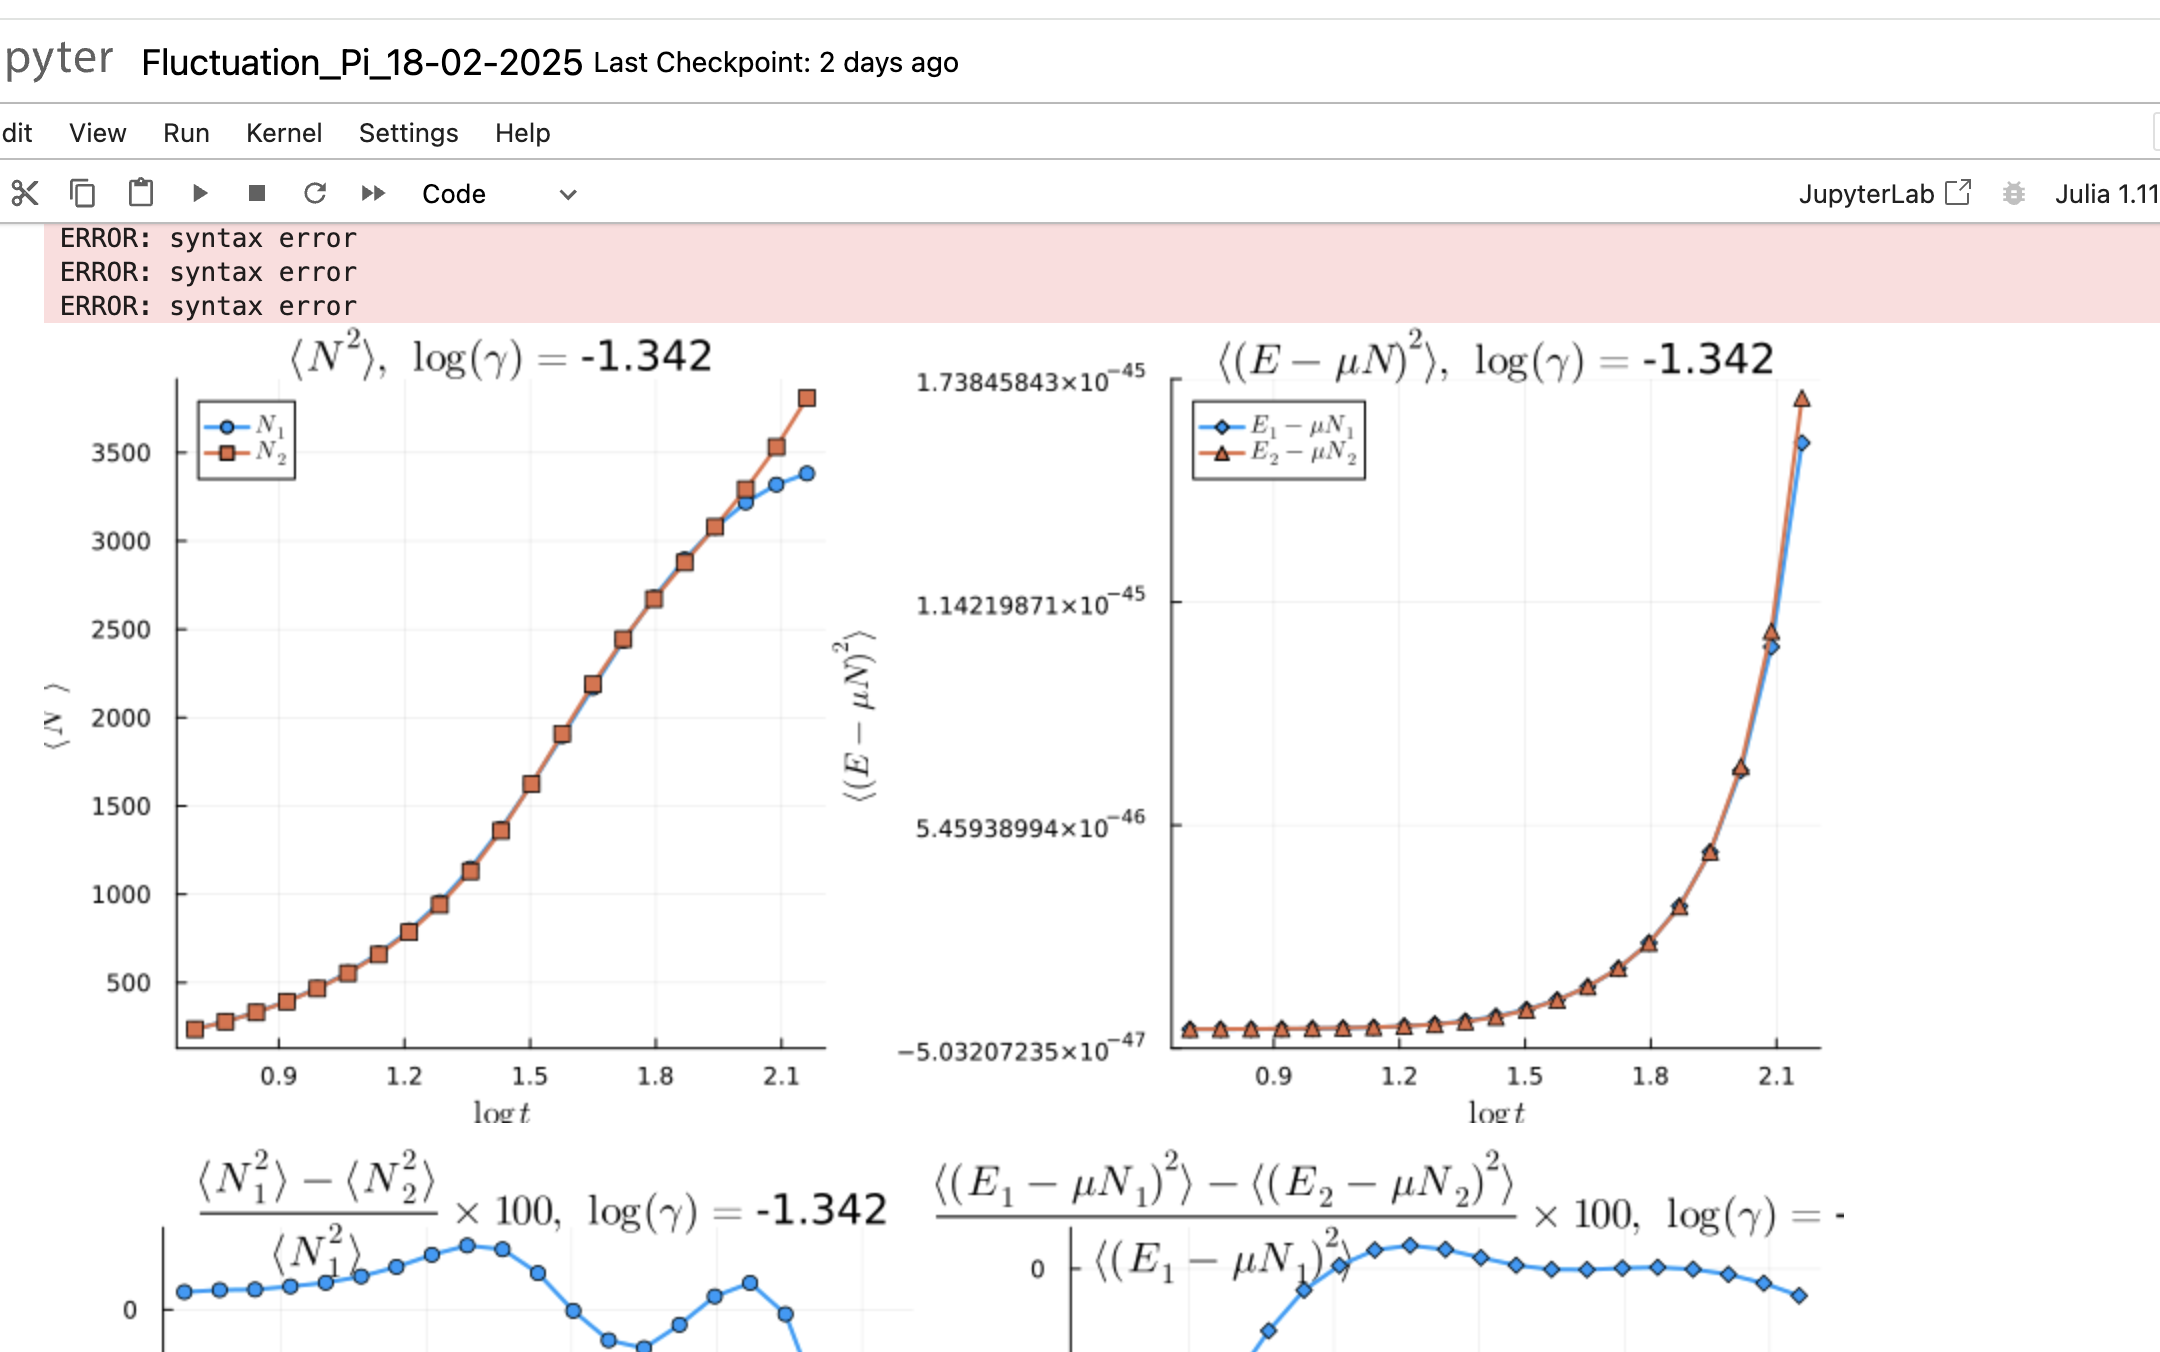
\includegraphics[width=1\textwidth]{Figures/test}

%\begin{aff}
%Donc une a l'ordre un en $\delta \theta (\operator{A}^{(0)})^{-1} %\operator{V}$ 

%\begin{eqnarray*}
%	\langle \delta \Pi ( \theta) \delta \Pi ( \theta') \rangle & = &  ( (\Pi^c_s - \Pi^c)\Pi^c/\Pi^c_s ) ( \theta ) \delta_{\theta, \theta'}/\delta \theta + \mathscr{F}(\theta , \theta' ) ,	
%\end{eqnarray*}

%avec 

%\begin{eqnarray*}
%	\mathscr{F}(\theta , \theta' ) & = & \left [ (\Pi^c_s - \Pi^c )( \theta)  +  (\Pi^c_s - \Pi^c ) ( \theta' )\right ] \frac{\Pi^c}{\Pi^c_s}(\theta)\frac{\Pi^c}{\Pi^c_s}(\theta') \frac{ \Delta( \theta'- \theta )}{ 2 \pi }\\
%	&&  - \left [ (\Pi^c_s - \Pi^c )( \theta)   (\Pi^c_s - \Pi^c ) ( \theta' )\right ] \frac{\Pi^c}{\Pi^c_s}(\theta)\frac{\Pi^c}{\Pi^c_s}(\theta')\int d\theta'' \left (   \frac{ \Pi^c/\Pi^c_s}{\Pi^c_s - \Pi^c} \right )(\theta'') \frac{\Delta(\theta''- \theta)}{2 \pi}\frac{\Delta(\theta''- \theta')}{2 \pi}  	
%\end{eqnarray*}
%\end{aff}



 









	